\section{Устойчивость Солнца и звезд. Термоядерные реакции.}

\subsection{Устойчивость Солнца и звезд}

Солнце, как и в целом большая часть звезд, устойчивые объекты по следующей причине. В нем действуют две основные силы, это гравитация, которая стремится его сжать, и силы давления, которые этому противодействуют. Сила давления существуют, потому что Солнце, в первую очередь, внутри горячее, идет процесс выделения энергии, и поэтому давление - это просто давление газа плюс давление излучения. Соответственно силы давления уравновешивают гравитацию и возникает красивый эффект саморегуляции.

Если под каким-то внешним воздействием Солнце поджалось, значит в центре возросла температура, поскольку вы сжимаете газовый шар, он нагревается. Возросла температура, возросла плотность, пошли термоядерные реакции. Но это хороший реактор, выделяется больше энергии, увеличивается давление и звезда начинает расширяться, она сама регулируется, вырастают силы давления, звезда расширяется, остывает, при этом падает плотность и снова устанавливается равновесие.

Благодаря этому механизму Солнце, как и остальные звезды, очень стабильный объект, находящийся в гидростатическом равновесии, которое очень трудно нарушить.


%Чтобы билет уж не был совсем пустым, давайте что-нибудь выведем. Например, можно записать уравнение для внутреннего устройства и попробовать оценить термодинамические величины в солнечных недрах, например, можно оценить давление и температуру.
%
%\begin{equation}
%	F_{gr} + F_p = 0
%\end{equation}
%
%Распишем силы:
%
%\begin{align}
%	F_p = F(r) - F(r + dr) = P(r) dS -F(r + dRr) dS = - \frac{dP}{dr} dr dS\\
%	F_{gr} = \frac{G M(r) m}{r^2}, \quad m = \rho dV
%\end{align}
%
%Подставим, получим:
%
%\begin{equation}
%	-\frac{dP}{dr} = \frac{G M}{r^2} \rho \qrq 
%\end{equation}


\subsection{Термоядерные реакции}

Будем говорить о звездах главной последовательности. Для них в принципе существует два основных цикла, по которым идут термоядерные реакции, это \textbf{протон-протонный цикл}, в ходе которого водород превращается гелий (доминирует в случае звезд, находящихся на главной последовательности и имеющих массу меньше или порядка Солнечной), и \textbf{CNO-цикл} (или его простой брат \textbf{CNO-I-цикл}), в котором превращение водорода в гелий происходит под воздействием катализаторов: углерода C и азота N.

\subsubsection{Протон-протонный цикл}

Рассмотрим на примере pp\RN{1} цепочки, которая самая частая. Все возможные цепочки приведены на рисунке \ref{fig:6_pp}.

Цикл состоит из трех стадий. Сперва два протона сливаются и образуют дейтрон, позитрон и электронное нейтрино. После этого дейтрон сливается с протоном и образует ядро \ce{^3He}. Наконец, сливаются два ядра гелия-3 и появляется ядро атома гелия-4 с высвобождением двух протонов. Итого:

\begin{align}
	\ce{p + p &-> ^2H + e^+ + \nu_e + E}\\
	\ce{^2H + p &-> ^3He + \gamma + E}\\
	\ce{^3He + ^3He &-> ^4He + 2p + E}
\end{align}

\begin{figure}[H]
	\centering
	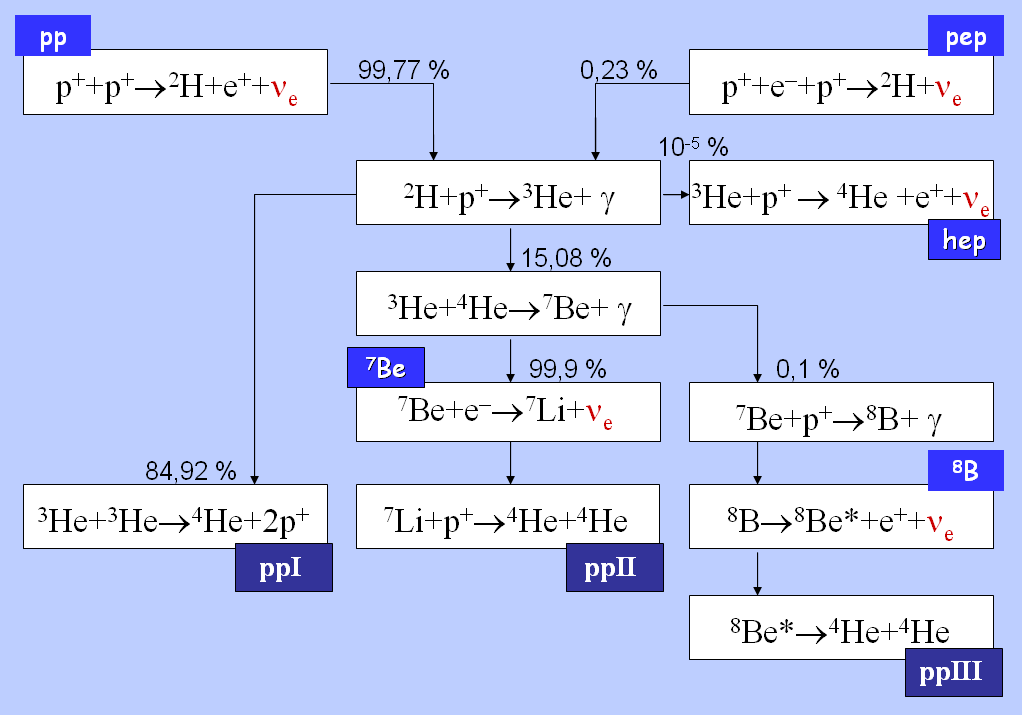
\includegraphics[width=0.7\linewidth]{6_pp}
	\caption{Три цепочки протон-протонного цикла, а также различные ветви}
	\label{fig:6_pp}
\end{figure}

\subsubsection{CNO-I-цикл}

Цикл сложный, поэтому рассмотрим на примере CNO-\RN{1}. Стадии такие:

\begin{align}
	\ce{^{12}C + p &-> ^{13}N + \gamma}\\
	\ce{^{13}N &-> ^{13}C + e^+ + \nu_e}\\
	\ce{^{13}C + p &-> ^{14}N + \gamma}\\
	\ce{^{14}N + p &-> ^{15}O + \gamma}\\
	\ce{^{15}O &-> ^{15}N + e^+ + \nu_e}\\
	\ce{^{15}N + p &-> ^{12}C + ^4He}
\end{align}

Картинка \ref{fig:6_CNO} для иллюстрации.

\begin{figure}[H]
	\centering
	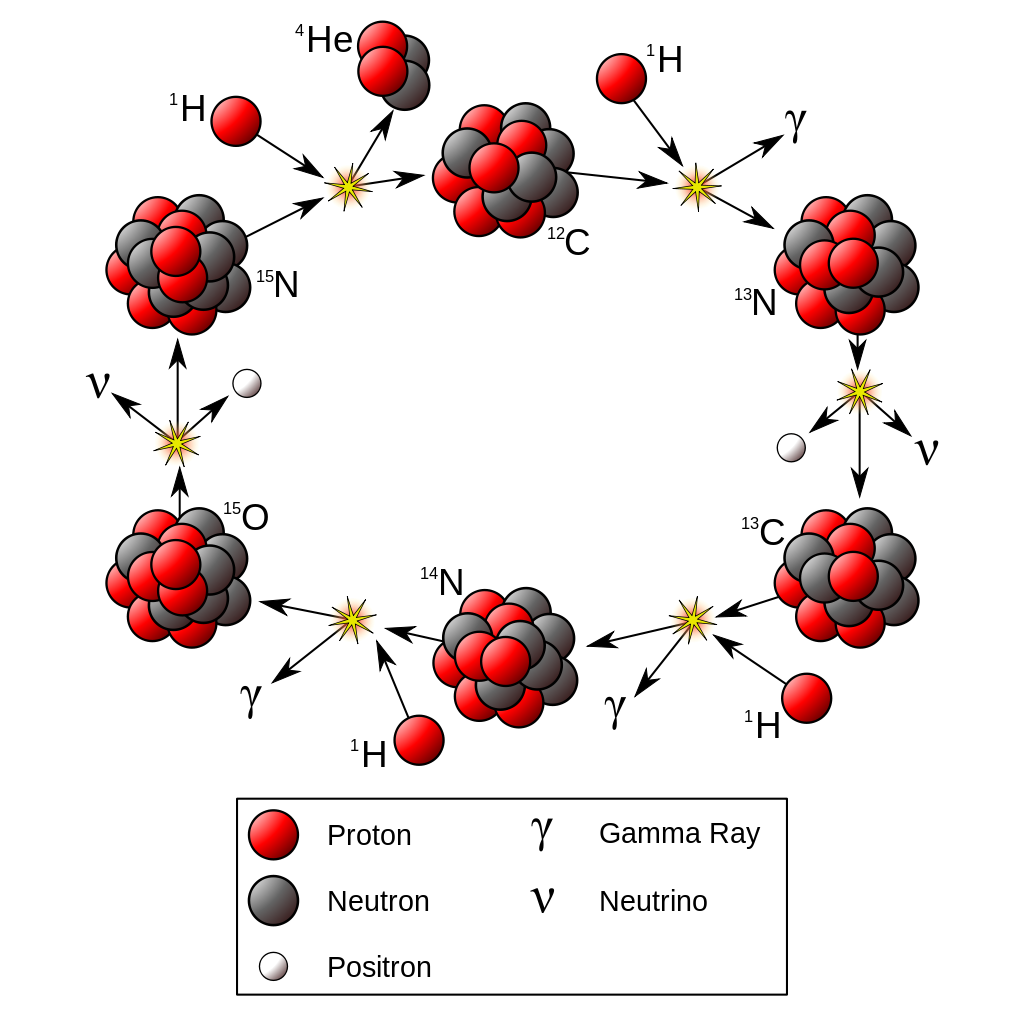
\includegraphics[width=0.7\linewidth]{6_CNO}
	\caption{Цикл \ce{CNO}-I}
	\label{fig:6_CNO}
\end{figure}

Есть прямо вот СВЕЖИЕ данные о том, что Солнце действительно работает по CNO: \href{https://arxiv.org/abs/2006.15115}{First Direct Experimental Evidence of CNO neutrinos} (от 26 июня 2020).

%\subsection{Синтез}
%
%Я не очень понимаю о чем тут еще говорить, но получается маловато, так что давайте еще про синтез поговорим.
%
%Вопрос: откуда элементы? Ответ ниже.
%
%Водород и гелий имеют космологическое происхождение, они составляли первичный газ во Вселенной. 
%
%Уникальные в своем роде \ce{Li}, \ce{Be}, \ce{B} могут производиться реакцией скалывания, когда у нас есть тяжелые ядра и космические лучи, которые могут их раскалывать и делать \ce{Be}, \ce{B}, которые в обычных циклах синтеза проходятся мимо.
%
%Все более массивное происходит от звезд. Не самые массивные элементы могут происходить от взрывов массивных звезд (коллапсирует ядро, сверхновая и новые элементы синтезируются), или от термоядерных взрывов белых карликов (обычно до группы железа). Более массивное может происходить, например, от слияния нейтронных звезд (это редко, но именно от них самые тяжелые элементы синтезируются).
%
%В чем вообще цимес, в том, что обычно это все в ядрах и остается (либо в белом карлике, либо вообще коллапсирует в черную дыру в случае массивных звезд), так что нам нужны какие-то процессы, которые могут выбрасывать элементы. Для этого есть два основных процесса: \textbf{S-процесс} и \textbf{R-процесс}.
%
%В случае S-процесса нейтроны залезают внутрь ядра и могут произвольно испытать бета-распад, повышая таким образом атомное число. Такой процесс идет например в оболочках звезд-гигантов.
%
%В чем проблема: при горении легких звезд мы доходим до кислорода, например, и получаем потом кислородно-углеродный белый карлик, т.е. просинтезированное вещество не выбрасывается. А тяжелые звезды хоть и идут до железа, но тоже не выдают это вещество в большинстве своем.